\documentclass[a4paper,11pt,twoside]{book}
\usepackage{listings}		
\usepackage{graphicx}
\usepackage[dvipsnames]{xcolor}
\usepackage{multicol}
\usepackage{adjustbox}
\usepackage{amssymb} 
\usepackage{amsmath}
\usepackage[ruled,vlined]{algorithm2e}
\usepackage{hyperref}
\hypersetup{
    colorlinks,
    citecolor=black,
    filecolor=black,
    linkcolor=black,
    urlcolor=black
}

\setlength{\tabcolsep}{1em}
\setlength{\emergencystretch}{10pt}
\graphicspath{ {./img/} }	
% \pagecolor{Periwinkle}
% \color{purple}				

\lstset{language=Java,						
	showspaces=false,
	showtabs=false,
	breaklines=true,
	showstringspaces=false,
	breakatwhitespace=true,
	commentstyle=\color{ForestGreen},
	keywordstyle=\color{blue},
	stringstyle=\color{red},
	identifierstyle=\color{Gray},
	basicstyle=\small\ttfamily
}

\newcommand{\bluetext}[1]{\textcolor{blue}{#1}}
\newcommand{\redtext}[1]{\textcolor{red}{#1}}
\newcommand{\orangetext}[1]{\textcolor{orange}{#1}}
\newcommand{\subtext}[1]{\textsubscript{#1}}
\newcommand{\supertext}[1]{\textsuperscript{#1}}
\newcommand{\Mod}[1]{\ (\mathrm{mod}\ #1)}

\begin{document}

\title{Appunti di Crittografia}
\author{Simone Ianniciello}
\date{A.A. 2020/2021}
\maketitle

\tableofcontents

\chapter{Introduzione}
\section{La crittologia}
La crittografia e' lo studio delle tecniche matematiche per:
\begin{description}
    \item[Crittografia] Metodi di cifratura.
    \item[Crittoanalisi] Metodi di interpretazione. 
\end{description}
\begin{center}
    Crittografia + Crittoanalisi = \textbf{Crittologia}
\end{center}
\subsection{Scenario}
A vuole spedire un messaggio a B, ma E sta' ascoltando il messaggio.
Per proteggere la comunicazione, A e B utilizzano dei metodi di cifratura.
\subsection{Cifratura}
\begin{tabular}{l | l}
    MSG & Insieme dei messaggi in chiaro\\
    CRITTO & Insieme dei crittogrammi\\
    C: MSG $\rightarrow$ CRITTO & Funzione di crittazione.\\
    D: CRITTO $\rightarrow$ MSG & Funzione di decrittazione.
\end{tabular}
C e D sono una l'inversa dell'altra: $D(c) = D(C(m)) = m$\newline
C e' iniettiva (messaggi diversi corrispondono a crittogrammi diversi).
% \section{Cifrari storici}
% Scitale:
% \includegraphics[width=20em]{scitale}\newline
% Cifrario di cesare:
% Ogni lettera del messaggio e' sostituita con quella 3 posizioni piu' avanti nell'alfabeto.
% 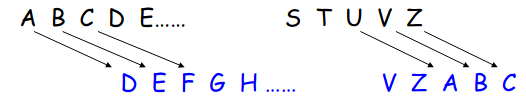
\includegraphics[width=20em]{cesare}\newline
\section{Classificazione dei cifrari}
I cifrari si dividono in:
\begin{description}
    \item[Cifrari per uso ristretto] Le funzioni C e D devono essere {\color{red}segrete}; Poco pratici per la crittografia \textit{di massa}.
    \item[Cifrari per uso generale] Si basano su un metodo a {\color{blue}chiave}. C e D sono pubbliche ma la chiave deve essere nota ai soli interessati del messaggio.
\end{description}
\subsection{Cifrari per uso generale}
Le definizioni di C e D diventano:

\begin{tabular}{l}
    C: MSG * KEYS $\rightarrow$ CRITTO\\
    D: CRITTO * KEYS $\rightarrow$ MSG\\
\end{tabular}

Se un crittoanalista entra in possesso di una chiave, basta cambiarla.
Esempi di cifrari a chiave segreta: 3DES, RC5, IDEA, AES.

\paragraph{Attacco esauriente (bruteforce)} Il crittoanalista dovrebbe provare tutte le chiavi finché non trova quella giusta per decrittare il messaggio.
Quasi impossibile da effettuare su chiavi abbastanza grandi ($>$20chars).
\section{Attacchi}
Gli attacchi possono avere successo completo (Si scopre la funzione D, compresa di chiave), oppure possono avere successo limitato (Si scopre solo qualche informazione su un messaggio).
\subsection{Attacchi al sistema crittografico}
\begin{tabular}{l | p{17em}}
    Cypher Text Attack & Il crittoanalista rileva una serie di crittogrammi $c_1, \dots, c_r$.\\
    Known Plain-Text Attack & Il crittoanalista conosce una serie di coppie $(c_1, m_1), \dots, (c_r, m_r)$.\\
    Chosen Plain-Text Attack & Il crittoanalista sceglie una serie di $m_1, \dots, m_r$ e si procura i relativi $c_1, \dots, c_m$.
\end{tabular}
\subsection{Attacchi Man-In-The-Middle MITM}
Il crittoanalista si inserisce nel canale di comunicazione e blocca tutti i messaggi diretti.
Puo' anche sostituire i messaggi originali con dei messaggi propri.
\begin{center}
    \begin{tabular}{c | c}
        Condizione normale & Attacco MITM\\
        $A \rightleftarrows B$ & $A \rightleftarrows E \rightleftarrows B$
    \end{tabular}
\end{center}

\section{Cifrari perfetti}
I cifrari perfetti sono totalmente sicuri, ma richiedono operazioni molto complesse perciò sono usati solo in condizioni estreme.
In essi $m$ e $c$ sono totalmente scorrelati tra loro.
\subsection{One-Time Pad}
E un cifrario perfetto ma ha svantaggi enormi che lo rendono quasi inutilizzabile:
\begin{itemize}
    \item Richiedono una chiave segreta nuova e perfettamente casuale per ogni messaggio.
    \item La chiave deve essere lunga quanto il messaggio.
\end{itemize}
\subsection{Cifrari sicuri}
I cifrari che vengono utilizzati ad ora non sono cifrari perfetti ma sono dichiarati sicuri. Cio' significa che non sono mai stati violati prima d'ora perché richiedono la risoluzione di problemi matematicamente difficili (Non essendo mai stato dimostrato $P \not\equiv NP$ non siamo \textit{certi} che siano inviolabili).
\section{Cifrari in uso}
\subsection{AES}
E' un \bluetext{cifrario simmetrico} (la stessa chiave viene utilizzata per crittare e decrittare), \bluetext{a blocchi} (il messaggio e' diviso in blocchi lunghi come il messaggio).
E' pubblicamente noto e utilizzato per comunicazioni \textit{non classificate}.
Si utilizzano chiavi brevi (128 o 256 bit).
\chapter{Esercizi}

\section{Correttezza RSA}

\begin{itemize}
    \item $p, q \mid m$
    \begin{itemize}
        \item Eulero: $a^{\Phi(n)} \equiv 1 \mod{n}$
        \item $e \times d \equiv 1 \mod{\Phi(n)} = 1 + r\Phi(n)$
        \item $m^{ed} \mod{n} \equiv m \times m^{r\Phi(n)} \mod{n} \equiv m \times (m^{\Phi(n)})^r \mod{n} \\\dequiv{Eul} m \times 1^r \mod{n} \equiv m \mod{n}$
    \end{itemize}
    \item $p \mid m \wedge q \nmid m$
    \begin{itemize}
        \item $m \equiv m^r \equiv 0 \mod{p} \implies (m^r - m) \equiv 0 \mod{p}$
        \item Eulero: $a^{\Phi(q)} \equiv 1 \mod{q}$
        \item $m^{ed} \mod{q} \equiv m^{1+r\Phi{n}} \mod{q} \equiv m \times m^{r(p-1)(q-1)} \mod{q} \\\equiv m \times (m^{\Phi(q)})^{r\Phi(p)} \mod{q} \equiv m \mod{q}$
        \item $(m^{ed} - m) \equiv 0 \mod{q} \implies (m^{ed} - m) \mid q$
        \item $(m^{ed} - m) \equiv 0 \mod{n} \implies m^{ed} \equiv m \mod{n}$
    \end{itemize}
\end{itemize}

\section{Cifrario perfetto}

\subsection{Definizione}

\begin{itemize}
    \item Un cifrario si dice perfetto se non \'e possibile inferire alcuna informazione sul messaggio originale, dato il crittogramma associato
    \item $\forall m \in Msg, c \in Critto, \pr(M = m) = \pr(M = m \mid C = c)$
    \item La conoscenza complessiva di un crittoanalista non cambia dopo aver letto il crittogramma in transito sul canale
\end{itemize}

\subsection{Enunciato di Shannon}

\begin{itemize}
    \item Dati $M$, l'insieme dei messaggi possibili e $K$, l'insieme delle chiavi
    \item Per Shannon : $|K| \geq |M|$
    \item Poniamo per assurdo che $|K| < |M|$
    \item Fissato un crittogramma $c \mid \pr(C = c) > 0$, esso corrisponde a $s \leq |K|$ messaggi (non necessariamente distinti) in M
    \item Dato che $s \leq |K| < |M|$ allora necessariamente esiste almeno un messaggio $m \mid \pr(M=m)>0$ non ottenibile da $c$
    \item Quindi $\pr(M=m \mid C=c) = 0 \not= \pr(M=m)$
\end{itemize}

\subsection{Perfettezza di One-Time Pad}

\begin{itemize}
    \item $\pr(M=m \mid C=c) = \dfrac{\pr(M=m,C=c)}{\pr(C=c)}$
    \item Per definizione di \m{XOR}, fissato $m$, chiavi diverse corrispondono a crittogrammi diversi
    \item Perci\`o $\pr(C = c) = (\nicefrac{1}{2})^n$ \'e costante
    \item Quindi gli eventi $(C=c) e (M=m)$ sono indipendenti
    \item Ne risulta che $\pr(M=m \mid C=c) = \dfrac{\pr(M=m) \times \cancel{\pr(C=c)}}{\cancel{\pr(C=c)}}$
\end{itemize}
\chapter{Orale}

\section{}
\chapter{Il ruolo del caso}

\section{Il significato algoritmico della casualità}

\begin{itemize}
    \item Casualità secondo Kolmogorov
    \begin{itemize}
        \item $\mathcal{K}$ : Complessità
        \item $S_i$ : Algoritmo
        \item $h$ : Sequenza "casuale"
        \item $p$ : Rappresentazione binaria dell'algoritmo
        \item $\mathcal{K}_{S_i}(h) = min\{|p| : S_i(p) = h\}$
    \end{itemize}
    \item Una sequenza \'e casuale se
    \begin{itemize}
        \item $\mathcal{K}(h) \geq |h| - \ceil{log_2(h)}$
    \end{itemize}
\end{itemize}

\subsection{Esistenza di sequenze casuali di lunghezza n}

\begin{itemize}
    \item $n$ : Lunghezza della rappresentazione binaria
    \item $S = 2^n$ : Tutte le sequenze binarie lunghe $n$
    \item Chiamiamo $T$ l'insieme delle sequenze non casuali all'interno di $S$
    \item $N = 2^{n \ceil{\log_2n} - 1}$ : Sequenze pi\'u corte di $n - \ceil{\log_2 n}$
    \item $N$ Contiene tutte anche tutti i programmi che generano le sequenze $T$
    \item $T \leq N < S$
    \item $\nicefrac{T}{S} < 2^{-\ceil{\log_2 n}}$ Tende a $0$ al crescere di $n$
\end{itemize}

\section{Generatori di numeri pseudo-casuali}

\begin{itemize}
    \item Generatore di numeri pseudo-casuali: algoritmo che parte da un piccolo valore iniziale detto seme e genera una sequenza arbitrariamente lunga di numeri.
    \item Proprietà di un generatore:
    \begin{itemize}
        \item \textbf{Frequenza} : Verifica se i diversi elementi appaiono in S approssimativamente lo stesso numero di volte
        \item \textbf{Poker} : Verifica la equidistribuzione di sottosequenze di lunghez\-za arbitraria ma prefissata
        \item \textbf{Autocorrelazione} : he verifica il numero di elementi ripetuti a distanza prefissata
        \item \textbf{Run} : verifica se le sottosequenze massimali contenenti elementi tutti uguali hanno una distribuzione esponenziale negativa
        \item \textbf{Prossimo bit} : Non esiste un algoritmo polinomiale in grado di predire l'(\textit{i} + 1)-esimo bit della sequenza conoscendo i bit precedenti
    \end{itemize} 
    \item Generatore BBS : $x_i \leftarrow (x_{i-1})^2 \text{ mod }n \wedge b_i = 1 \Leftrightarrow x_{m-i}$ e' dispari
\end{itemize}

\section{Algoritmi randomizzati}

\begin{itemize}
    \item \textit{Las Vegas} : Risultato \textbf{sicuramente} corretto in tempo \textbf{probabilmente} breve
    \item \textit{Monte Carlo} : Risultato \textbf{probabilmente} corretto in tempo \textbf{sicuramente} breve
    \item \textit{Miller e Rabin} : Algoritmo di tipo \textit{Monte Carlo} per il controllo di un numero primo
    \begin{itemize}
        \item $n$ : Valore da controllare
        \item $z$ : Intero tale che $z = \dfrac{N - 1}{2^w}$
        \item $y$ : $y \in [2, N-1]$ 
        \item P\textsubscript{1} : $mcd(N, y) = 1$
        \item P\textsubscript{2} : $(y^z \mod{N} = 1) \vee (\exists{i}, 0 \leq i \leq w-1 : y^{2^iz} \mod{N} = -1)$
        \item $(P_1 \wedge P_2) = false$ : N \'e sicuramente composto
        \item $(P_1 \wedge P_2) = true$ : N \'e primo con probabilità $p \geq \dfrac{3}{4}$
    \end{itemize}
\end{itemize}
\chapter{Esempi di algoritmi numerici}
\section{Euclide}
\[ a,b \in \mathbb{Z}, a \geq b, a > 0 \]
\begin{equation*}
    MCD(a,b) =
    \begin{cases}
        a &\text{ se } b=0\\
        MCD(b, a\Mod{b} &\text{ se } b\neq0)
    \end{cases}
\end{equation*}
Numero di passi: $O(log(a))$
\subsection{Dimostrazione}
\[ a\Mod{b} \leq \dfrac{a}{2} \]
Questo perché
\begin{equation*}
    \begin{split}
        a &\\
        & =\\
        & qb + a\Mod{b}\\
        (q = \dfrac{a}{b} \wedge a \geq b) & \geq\\
        & b + a\Mod{b}\\
        b > a\Mod{b} & >\\
        & 2a\Mod{b}
    \end{split}
\end{equation*}
Costo di MCD: $O(n^3)$
% TODO: Che cazzo e' sta roba?? ALGO di nuovo?!?
\newpage
\section{Test di primalità (inefficiente)}
\begin{algorithm*}
    \For($\sqrt{N}$: Max divisore se N non e' primo){$i=2$; $i < \sqrt{N}$; $i$++} {
        \If{$N \% i == 0$} {
            return false;
        }
    }
    return true;
    \caption{Primo(N)}
\end{algorithm*}

\end{document}